\PassOptionsToPackage{unicode=true}{hyperref} % options for packages loaded elsewhere
\PassOptionsToPackage{hyphens}{url}
\PassOptionsToPackage{dvipsnames,svgnames*,x11names*}{xcolor}
%
\documentclass[]{book}
\usepackage{lmodern}
\usepackage{amssymb,amsmath}
\usepackage{ifxetex,ifluatex}
\usepackage{fixltx2e} % provides \textsubscript
\ifnum 0\ifxetex 1\fi\ifluatex 1\fi=0 % if pdftex
  \usepackage[T1]{fontenc}
  \usepackage[utf8]{inputenc}
  \usepackage{textcomp} % provides euro and other symbols
\else % if luatex or xelatex
  \usepackage{unicode-math}
  \defaultfontfeatures{Ligatures=TeX,Scale=MatchLowercase}
\fi
% use upquote if available, for straight quotes in verbatim environments
\IfFileExists{upquote.sty}{\usepackage{upquote}}{}
% use microtype if available
\IfFileExists{microtype.sty}{%
\usepackage[]{microtype}
\UseMicrotypeSet[protrusion]{basicmath} % disable protrusion for tt fonts
}{}
\IfFileExists{parskip.sty}{%
\usepackage{parskip}
}{% else
\setlength{\parindent}{0pt}
\setlength{\parskip}{6pt plus 2pt minus 1pt}
}
\usepackage{xcolor}
\usepackage{hyperref}
\hypersetup{
            pdftitle={Einführung in die mathematische Datenanalyse},
            pdfauthor={Jan Heiland},
            colorlinks=true,
            linkcolor=Maroon,
            filecolor=Maroon,
            citecolor=Blue,
            urlcolor=purple,
            breaklinks=true}
\urlstyle{same}  % don't use monospace font for urls
\usepackage{color}
\usepackage{fancyvrb}
\newcommand{\VerbBar}{|}
\newcommand{\VERB}{\Verb[commandchars=\\\{\}]}
\DefineVerbatimEnvironment{Highlighting}{Verbatim}{commandchars=\\\{\}}
% Add ',fontsize=\small' for more characters per line
\usepackage{framed}
\definecolor{shadecolor}{RGB}{248,248,248}
\newenvironment{Shaded}{\begin{snugshade}}{\end{snugshade}}
\newcommand{\AlertTok}[1]{\textcolor[rgb]{0.94,0.16,0.16}{#1}}
\newcommand{\AnnotationTok}[1]{\textcolor[rgb]{0.56,0.35,0.01}{\textbf{\textit{#1}}}}
\newcommand{\AttributeTok}[1]{\textcolor[rgb]{0.77,0.63,0.00}{#1}}
\newcommand{\BaseNTok}[1]{\textcolor[rgb]{0.00,0.00,0.81}{#1}}
\newcommand{\BuiltInTok}[1]{#1}
\newcommand{\CharTok}[1]{\textcolor[rgb]{0.31,0.60,0.02}{#1}}
\newcommand{\CommentTok}[1]{\textcolor[rgb]{0.56,0.35,0.01}{\textit{#1}}}
\newcommand{\CommentVarTok}[1]{\textcolor[rgb]{0.56,0.35,0.01}{\textbf{\textit{#1}}}}
\newcommand{\ConstantTok}[1]{\textcolor[rgb]{0.00,0.00,0.00}{#1}}
\newcommand{\ControlFlowTok}[1]{\textcolor[rgb]{0.13,0.29,0.53}{\textbf{#1}}}
\newcommand{\DataTypeTok}[1]{\textcolor[rgb]{0.13,0.29,0.53}{#1}}
\newcommand{\DecValTok}[1]{\textcolor[rgb]{0.00,0.00,0.81}{#1}}
\newcommand{\DocumentationTok}[1]{\textcolor[rgb]{0.56,0.35,0.01}{\textbf{\textit{#1}}}}
\newcommand{\ErrorTok}[1]{\textcolor[rgb]{0.64,0.00,0.00}{\textbf{#1}}}
\newcommand{\ExtensionTok}[1]{#1}
\newcommand{\FloatTok}[1]{\textcolor[rgb]{0.00,0.00,0.81}{#1}}
\newcommand{\FunctionTok}[1]{\textcolor[rgb]{0.00,0.00,0.00}{#1}}
\newcommand{\ImportTok}[1]{#1}
\newcommand{\InformationTok}[1]{\textcolor[rgb]{0.56,0.35,0.01}{\textbf{\textit{#1}}}}
\newcommand{\KeywordTok}[1]{\textcolor[rgb]{0.13,0.29,0.53}{\textbf{#1}}}
\newcommand{\NormalTok}[1]{#1}
\newcommand{\OperatorTok}[1]{\textcolor[rgb]{0.81,0.36,0.00}{\textbf{#1}}}
\newcommand{\OtherTok}[1]{\textcolor[rgb]{0.56,0.35,0.01}{#1}}
\newcommand{\PreprocessorTok}[1]{\textcolor[rgb]{0.56,0.35,0.01}{\textit{#1}}}
\newcommand{\RegionMarkerTok}[1]{#1}
\newcommand{\SpecialCharTok}[1]{\textcolor[rgb]{0.00,0.00,0.00}{#1}}
\newcommand{\SpecialStringTok}[1]{\textcolor[rgb]{0.31,0.60,0.02}{#1}}
\newcommand{\StringTok}[1]{\textcolor[rgb]{0.31,0.60,0.02}{#1}}
\newcommand{\VariableTok}[1]{\textcolor[rgb]{0.00,0.00,0.00}{#1}}
\newcommand{\VerbatimStringTok}[1]{\textcolor[rgb]{0.31,0.60,0.02}{#1}}
\newcommand{\WarningTok}[1]{\textcolor[rgb]{0.56,0.35,0.01}{\textbf{\textit{#1}}}}
\usepackage{longtable,booktabs}
% Fix footnotes in tables (requires footnote package)
\IfFileExists{footnote.sty}{\usepackage{footnote}\makesavenoteenv{longtable}}{}
\usepackage{graphicx,grffile}
\makeatletter
\def\maxwidth{\ifdim\Gin@nat@width>\linewidth\linewidth\else\Gin@nat@width\fi}
\def\maxheight{\ifdim\Gin@nat@height>\textheight\textheight\else\Gin@nat@height\fi}
\makeatother
% Scale images if necessary, so that they will not overflow the page
% margins by default, and it is still possible to overwrite the defaults
% using explicit options in \includegraphics[width, height, ...]{}
\setkeys{Gin}{width=\maxwidth,height=\maxheight,keepaspectratio}
\setlength{\emergencystretch}{3em}  % prevent overfull lines
\providecommand{\tightlist}{%
  \setlength{\itemsep}{0pt}\setlength{\parskip}{0pt}}
\setcounter{secnumdepth}{5}
% Redefines (sub)paragraphs to behave more like sections
\ifx\paragraph\undefined\else
\let\oldparagraph\paragraph
\renewcommand{\paragraph}[1]{\oldparagraph{#1}\mbox{}}
\fi
\ifx\subparagraph\undefined\else
\let\oldsubparagraph\subparagraph
\renewcommand{\subparagraph}[1]{\oldsubparagraph{#1}\mbox{}}
\fi

% set default figure placement to htbp
\makeatletter
\def\fps@figure{htbp}
\makeatother

\usepackage[]{natbib}
\bibliographystyle{plainnat}

\title{Einführung in die mathematische Datenanalyse}
\author{Jan Heiland}
\providecommand{\institute}[1]{}
\institute{FAU Erlangen-Nürnberg}
\date{FAU Erlangen-Nürnberg -- Sommersemester 2022}

\begin{document}
\maketitle

{
\hypersetup{linkcolor=}
\setcounter{tocdepth}{1}
\tableofcontents
}
\hypertarget{vorwort}{%
\chapter*{Vorwort}\label{vorwort}}
\addcontentsline{toc}{chapter}{Vorwort}

Das ist ein Aufschrieb.

Korrekturen und Wünsche immer gerne als \emph{issues} oder \emph{pull requests} ans \href{https://github.com/highlando/script-emds}{github-repo}.

\hypertarget{was-ist-data-science}{%
\chapter{Was ist Data Science?}\label{was-ist-data-science}}

Data Science umfasst unter anderem folgende Aufgaben:

\begin{enumerate}
\def\labelenumi{\arabic{enumi}.}
\item
  Strukturieren/Aufbereiten (Umgehen mit falschen, korrumpierten, fehlenden,
  unformatierten Daten)
\item
  Data Exploration (Daten ``verstehen'')
\item
  Data Analysis (quantitative Analysen, Hypothesen aufstellen)
\item
  Data Visualization (Hypothesen graphisch kommunizieren)
\item
  Modelle erzeugen/validieren (Regeln/Muster erkennen, Vorhersagen treffen) -- \emph{das} ist Machine Learning aber es gibt auch viele andere Ansätze.
\item
  Daten Reduktion
\end{enumerate}

\hypertarget{wie-passiert-die-datenanalyse}{%
\section{Wie passiert die Datenanalyse?}\label{wie-passiert-die-datenanalyse}}

Mit mathematischen Methoden aus den Bereichen der

\begin{itemize}
\tightlist
\item
  linearen Algebra (z.B. Matrizen, Basen, lineare Gleichungssysteme)
\item
  Statistik (z.B. Mittelwerte, Korrelationen, Verteilungen)
\item
  Analysis (Grenzwerte, Abschätzungen)
\item
  \ldots{}
\end{itemize}

Dabei hilft Software, z.B.,

\begin{itemize}
\tightlist
\item
  Excel
\item
  \textbf{Python}
\item
  Matlab
\item
  R
\end{itemize}

bei der Berechnung, Automatisierung, Visualisierung.

\begin{quote}
Python ist ein de-facto Standard in Data Science und Machine Learning.
\end{quote}

\hypertarget{was-sind-daten}{%
\section{Was sind Daten?}\label{was-sind-daten}}

Wie sehen Daten aus?

\begin{itemize}
\item
  Numerisch reell, z.B. Temperatur
\item
  Numerisch diskret, z.B. Anzahl
\item
  Ordinal: Element einer festen Menge mit expliziter Ordnung, z.B.
  \{neuwertig, mit Gebrauchsspuren, defekt\}
\item
  Binär: Eine von zwei Möglichkeiten, z.B. Wahr/Falsch oder aktiv/inaktiv
\item
  Kategoriell: Element einer festen Menge ohne klare Ordnung, z.B.
  \{Säugetier, Vogel, Fisch\}
\item
  sonstige strukturierte Daten, z.B. geographische Daten, Graphen
\item
  reiner Text, z.B. Freitext in Restaurantbewertung
\end{itemize}

Außerdem können wir noch allgemeine Eigenschaften (Qualitätsmerkmale) von Daten unterscheiden

\begin{itemize}
\tightlist
\item
  strukturiert
\item
  lückenhaft
\item
  fehlerbehaftet (\emph{verrauscht})
\item
  interpretierbar
\item
  geordnet (oder nicht zu ordnen)
\end{itemize}

\hypertarget{beispiele}{%
\section{Beispiele}\label{beispiele}}

\hypertarget{tabellendaten-mietpreise}{%
\subsection{Tabellendaten -- Mietpreise}\label{tabellendaten-mietpreise}}

\begin{figure}
\centering
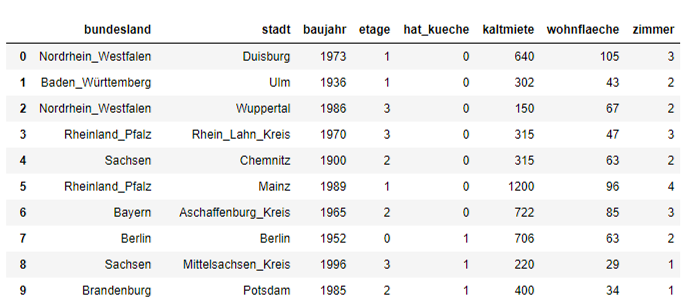
\includegraphics{bilder/dataframe.png}
\caption{Abbildung: Tabelle von Wohnungsangeboten}
\end{figure}

Hier wären die Aufgaben von Data Science:

\begin{itemize}
\tightlist
\item
  Daten ``verstehen'', Zusammenhänge zwischen
  Variablen aufdecken,
\item
  visualisieren.
\item
  Gegebenenfalls fehlende Einträge bei (z.B.) \texttt{kaltmiete} vorhersagen
\end{itemize}

\begin{figure}
\centering
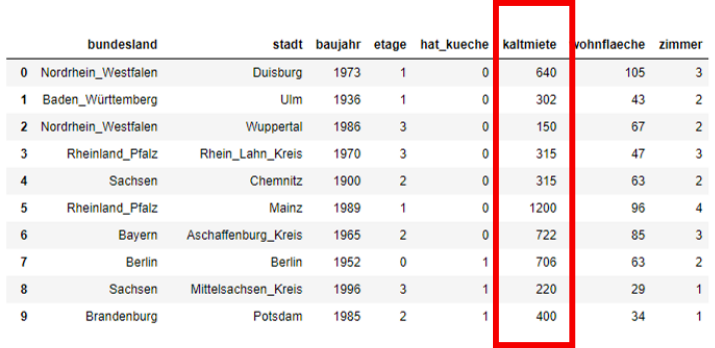
\includegraphics{bilder/dataframe_spalte.png}
\caption{Abbildung: Eine Spalte der Tabelle}
\end{figure}

Datenexploration und -analyse für einzelne Variablen 1/3 Wir betrachten
eine \emph{numerische} Variable in einem rechteckigen Datensatz, also eine
\emph{Spalte} (z.B. \texttt{kaltmiete}). Wir bezeichnen den \(i\)-ten Eintrag in
dieser Spalte mit \(x_i\), wobei \(i=1,\ldots,N\) (\(N\) Anzahl der Zeilen).

Folgende \emph{Schätzer}/\emph{Metriken} können dabei helfen, diese Spalte besser
zu verstehen:

\begin{itemize}
\item
  Mittelwert \(\overline x= \frac1 N\sum_{i=1}^N x_i\)
\item
  gewichteter Mittelwert
  \(\overline x_w = \frac{\sum_{i=1}^N w_i x_i}{\sum_{j=1}^N w_j}\),
  wobei \(w_i\) das Gewicht des \(i\)-ten Eintrages ist (z.B. eine andere
  Variable).
\item
  Varianz: \(s_x^2 = \frac{1}{N-1} \sum_{i=1}^N (x_i-\overline x)^2\)
\item
  Standardabweichung \(s = \sqrt{s_x^2}\).
\item
  Median = \(\frac{315 + 400}{2} = 357.5\).
\end{itemize}

Datenexploration und -analyse für mehrere Variablen Wir betrachten zwei
Spalten \(x = (x_1,\ldots,x_N)\) und \(y = (y_1,\ldots, y_N)\).\\

Das Verteilung von zwei Variablen läßt sich im sogenannte \textbf{Scatter Plot} visualisieren.

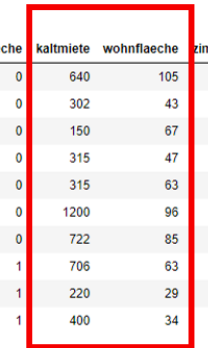
\includegraphics[width=0.27\textwidth,height=\textheight]{bilder/dataframe_spalte3.png}
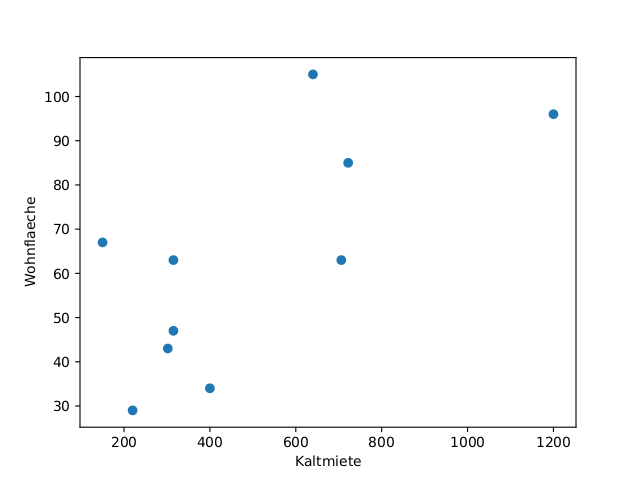
\includegraphics[width=0.7\textwidth,height=\textheight]{bilder/scatterplot.png}

Datenexploration und -analyse für mehrere Variablen Wir betrachten zwei
Spalten \(x = (x_1,\ldots,x_N)\) und \(y = (y_1,\ldots, y_N)\).

\begin{itemize}
\item
  Kovarianz
  \(s_{xy} = \frac{1}{N-1}\sum_{i=1}^N (x_i - \overline x)(y_i - \overline y)\)
\item
  Korrelation \(\rho_{xy} = \frac{s_{xy}}{s_x\cdot s_y} \in [-1,1]\).
\item
  \(\rho \approx 1\): Starke positive Korrelation, wenn \(x\) groß ist,
  ist \(y\) auch groß.
\item
  \(\rho \approx -1\): Starke negative Korrelation, wenn \(x\) groß ist,
  ist \(y\) klein
\item
  \(\rho \approx 0\): Wenig/keine Korrelation.
\end{itemize}

\begin{figure}
\centering
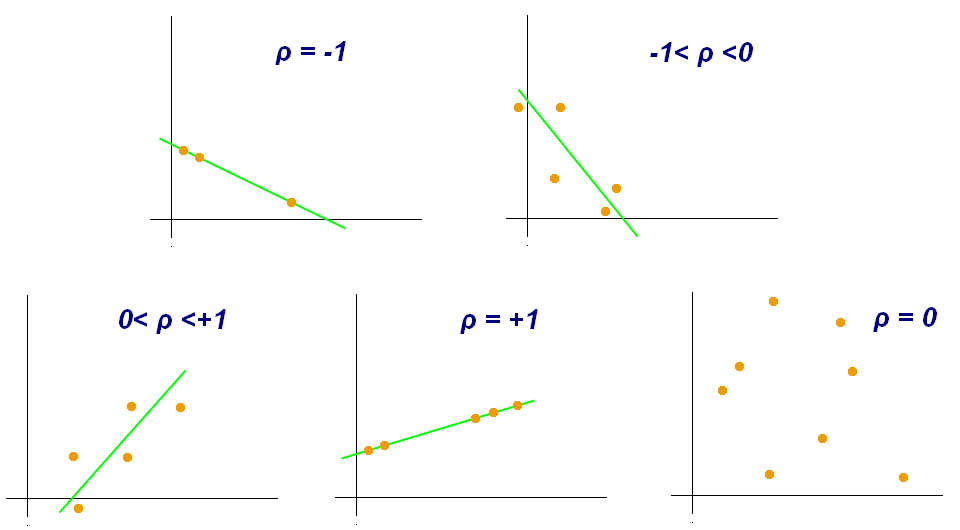
\includegraphics[width=0.65\textwidth,height=\textheight]{bilder/Correlation_coefficient.png}
\caption{Von Kiatdd - Eigenes Werk, CC BY-SA 3.0, \url{https://commons.wikimedia.org/w/index.php?curid=37108966}}
\end{figure}

\hypertarget{covid-19-daten}{%
\subsection{COVID-19 Daten}\label{covid-19-daten}}

Vergleiche die Einführung in \emph{Mathematik für Data Science 1} vom letzten Semester.

\hypertarget{netflix-prize}{%
\subsection{Netflix Prize}\label{netflix-prize}}

Hierbei geht es darum, ob aus bekannten Bewertungen von vielen verschiedenen Benutzern für viele verschiedene Filme abgeleitet werden kann, ob ein bestimmter Nutzer einen bestimmten Film mag (also positiv bewerten würde).

Vergleiche auch \href{https://en.wikipedia.org/wiki/Netflix_Prize}{Wikipedia:Netflix\_Prize}

Das (Trainings-)Daten bestehen über \texttt{480189} Benutzer, die für \texttt{17770} Filme insgesamt \texttt{100480507} Bewertungen als ganze Zahlen zwischen \texttt{1} und \texttt{5} verteilten.

Ziel der Datenanalyse war es, für \texttt{2817131} ``Paare'' von Benutzern und Filmen, die Bewertung vorauszusagen. Neben der schieren Masse an Daten kamen noch Einschränkungen hinzu, die ein Mindestmaß an Qualität der Vorhersage sicherstellen sollten.

Das Problem ließe sich wie folgt darstellen.

\begin{longtable}[]{@{}cccccc@{}}
\toprule
Benutzer \textbackslash{} Film & \texttt{F1} & \texttt{F2} & \texttt{...} & \texttt{Fn} & \texttt{...}\tabularnewline
\midrule
\endhead
\texttt{B1} & -- & 3 & \texttt{...} & 5 & \texttt{...}\tabularnewline
\texttt{B2} & 3 & 4 & \texttt{...} & 2 & \texttt{...}\tabularnewline
\texttt{B3} & 1 & 2 & \texttt{...} & \textbf{?} & \texttt{...}\tabularnewline
\texttt{...} & 3 & 4 & \texttt{...} & -- & \texttt{...}\tabularnewline
\bottomrule
\end{longtable}

Gegeben viele (aber bei weitem nicht alle) Einträge in einer riesigen Tabelle. Können wir aus den Zusammenhängen bestimmte fehlende Einträge (z.B. wie findet Nutzer \texttt{B3} den Film \texttt{Fn}) herleiten?

Die besten Lösungen für dieses Problem basieren durchweg auf \emph{Machine Learning} Ansätzen.

\hypertarget{python}{%
\section{Python}\label{python}}

Die Programmiersprache \texttt{python} wird uns durchs Semester begleiten. Einfach weil sie so wichtig ist für \emph{Data Science} aber auch weil sie (meiner Meinung nach) einfach zu erlernen und zu benutzen ist.

\hypertarget{aufgaben}{%
\section{Aufgaben}\label{aufgaben}}

\hypertarget{python-1}{%
\subsection{Python}\label{python-1}}

Bringen sie ihr \texttt{python} zum Laufen, installieren sie \texttt{numpy}, \texttt{scipy} und \texttt{matplotlib} und führen sie das folgende script aus.

\begin{Shaded}
\begin{Highlighting}[]
\ImportTok{import}\NormalTok{ numpy }\ImportTok{as}\NormalTok{ np}
\ImportTok{import}\NormalTok{ matplotlib.pyplot }\ImportTok{as}\NormalTok{ plt}

\NormalTok{N }\OperatorTok{=} \DecValTok{20}
\NormalTok{xmax }\OperatorTok{=} \DecValTok{2}
\NormalTok{xmin }\OperatorTok{=} \DecValTok{0}

\NormalTok{xdata }\OperatorTok{=}\NormalTok{ np.linspace(xmin, xmax, N)}
\NormalTok{ydata }\OperatorTok{=}\NormalTok{ np.exp(xdata)}

\NormalTok{plt.figure(}\DecValTok{1}\NormalTok{)}
\NormalTok{plt.plot(xdata, ydata, }\StringTok{'.'}\NormalTok{)}

\NormalTok{plt.figure(}\DecValTok{2}\NormalTok{)}
\NormalTok{plt.semilogy(xdata, ydata, }\StringTok{'.'}\NormalTok{)}
\NormalTok{plt.show()}
\end{Highlighting}
\end{Shaded}

\hypertarget{einheitsmatrix}{%
\subsection{Einheitsmatrix}\label{einheitsmatrix}}

Schreiben sie ein script, dass die \texttt{5x5} Einheitsmatrix auf 3 verschiedene Arten erzeugt. (Eine Art könnte die eingebaute \texttt{numpy} Funktion \texttt{eye} sein).

\begin{Shaded}
\begin{Highlighting}[]
\ImportTok{import}\NormalTok{ numpy }\ImportTok{as}\NormalTok{ np}

\NormalTok{idfive }\OperatorTok{=}\NormalTok{ np.eye(}\DecValTok{5}\NormalTok{)}
\BuiltInTok{print}\NormalTok{(idfive)}
\end{Highlighting}
\end{Shaded}

Hinweis: schauen sie sich mal an wie \texttt{numpy}'s \texttt{arrays} funktionieren.

\hypertarget{matrizen-multiplikation-und-potenz}{%
\subsection{Matrizen Multiplikation und Potenz}\label{matrizen-multiplikation-und-potenz}}

Schreiben sie ein script, das die Übungsaufgabe aus der Vorlesung (potenzieren der Matrizen \(M_i\), \(i=1,2,3,4\)) löst. Zum Beispiel mit

\begin{Shaded}
\begin{Highlighting}[]
\ImportTok{import}\NormalTok{ numpy }\ImportTok{as}\NormalTok{ np}
\NormalTok{mone }\OperatorTok{=}\NormalTok{ np.array([[}\FloatTok{0.9}\NormalTok{, }\FloatTok{0.9}\NormalTok{], [}\FloatTok{0.9}\NormalTok{, }\FloatTok{0.9}\NormalTok{]])}

\NormalTok{mone_ptwo }\OperatorTok{=}\NormalTok{ mone }\OperatorTok{@}\NormalTok{ mone}
\BuiltInTok{print}\NormalTok{(mone_ptwo)}

\NormalTok{mone_pfour }\OperatorTok{=}\NormalTok{ mone_ptwo }\OperatorTok{@}\NormalTok{ mone_ptwo}
\BuiltInTok{print}\NormalTok{(mone_pfour)}
\end{Highlighting}
\end{Shaded}

Oder so:

\begin{Shaded}
\begin{Highlighting}[]
\ImportTok{import}\NormalTok{ numpy }\ImportTok{as}\NormalTok{ np}
\NormalTok{mone }\OperatorTok{=}\NormalTok{ np.array([[}\FloatTok{0.9}\NormalTok{, }\FloatTok{0.9}\NormalTok{], [}\FloatTok{0.9}\NormalTok{, }\FloatTok{0.9}\NormalTok{]])}
\NormalTok{mone_p }\OperatorTok{=}\NormalTok{ np.eye(}\DecValTok{2}\NormalTok{)}

\ControlFlowTok{for}\NormalTok{ k }\KeywordTok{in} \BuiltInTok{range}\NormalTok{(}\DecValTok{16}\NormalTok{):}
\NormalTok{    mone_p }\OperatorTok{=}\NormalTok{ mone_p }\OperatorTok{@}\NormalTok{ mone}
    \ControlFlowTok{if}\NormalTok{ k }\OperatorTok{==} \DecValTok{1} \KeywordTok{or}\NormalTok{ k }\OperatorTok{==} \DecValTok{3} \KeywordTok{or}\NormalTok{ k }\OperatorTok{==} \DecValTok{15}\NormalTok{:}
        \BuiltInTok{print}\NormalTok{(}\StringTok{'k='}\NormalTok{, k}\OperatorTok{+}\DecValTok{1}\NormalTok{)}
        \BuiltInTok{print}\NormalTok{(mone_p)}
\end{Highlighting}
\end{Shaded}

Achtung:

\begin{itemize}
\tightlist
\item
  bei Matrizen kann auch \texttt{*} benutzt werden -- das ist aber nicht die richtige Matrizenmultiplikation (sondern die Multiplikation eintragsweise)
\item
  Moegliche Realisierung der Matrizenmultiplikation

  \begin{itemize}
  \tightlist
  \item
    \texttt{np.dot(A,\ B)} -- die klassische Methode
  \item
    \texttt{A.dot(B)} -- das selbe (manchmal besser, wenn \texttt{A} etwas allgemeiner ist (zum Beispiel eine \texttt{scipy.sparse} matrix)
  \item
    \texttt{A\ @\ B} -- convenience Notation
  \end{itemize}
\end{itemize}

\hypertarget{lineare-regression}{%
\chapter{Lineare Regression}\label{lineare-regression}}

Ein wesentlicher Aspekt von \emph{Data Science} ist die Analyse oder das
Verstehen von Daten. Allgemein gesagt, es wird versucht, aus den Daten
heraus Aussagen über Trends oder Eigenschaften des Phänomens zu treffen,
mit welchem die Daten im Zusammenhang stehen.

Wir kommen nochmal auf das Beispiel aus der Einführungswoche zurück, werfen eine bereits geschärften Blick darauf und gehen das mit verbesserten mathematischen Methoden an.

Gegeben seien die Fallzahlen aus der CoVID Pandemie 2020 für Bayern für den Oktober 2020.

\hypertarget{tab:covid-cases}{}
\begin{longtable}[]{@{}llllllllllll@{}}
\caption{Anzahl der SARS-CoV-2 Neuinfektionen in Bayern im Oktober 2020.}\tabularnewline
\toprule
Tag & 1 & 2 & 3 & 4 & 5 & 6 & 7 & 8 & 9 & 10 & 11\tabularnewline
\midrule
\endfirsthead
\toprule
Tag & 1 & 2 & 3 & 4 & 5 & 6 & 7 & 8 & 9 & 10 & 11\tabularnewline
\midrule
\endhead
Fälle & 352 & 347 & 308 & 151 & 360 & 498 & 664 & 686 & 740 & 418 & 320\tabularnewline
\bottomrule
\end{longtable}

\begin{longtable}[]{@{}lllllllllll@{}}
\toprule
Tag & 12 & 13 & 14 & 15 & 16 & 17 & 18 & 19 & 20 & 21\tabularnewline
\midrule
\endhead
Fälle & 681 & 691 & 1154 & 1284 & 127 & 984 & 573 & 1078 & 1462 & 2239\tabularnewline
\bottomrule
\end{longtable}

\begin{longtable}[]{@{}lllllllllll@{}}
\toprule
Tag & 22 & 23 & 24 & 25 & 26 & 27 & 28 & 29 & 30 & 31\tabularnewline
\midrule
\endhead
Fälle & 2236 & 2119 & 1663 & 1413 & 2283 & 2717 & 3113 & 2972 & 3136 & 2615\tabularnewline
\bottomrule
\end{longtable}

\begin{figure}
\hypertarget{fig:cases}{%
\centering
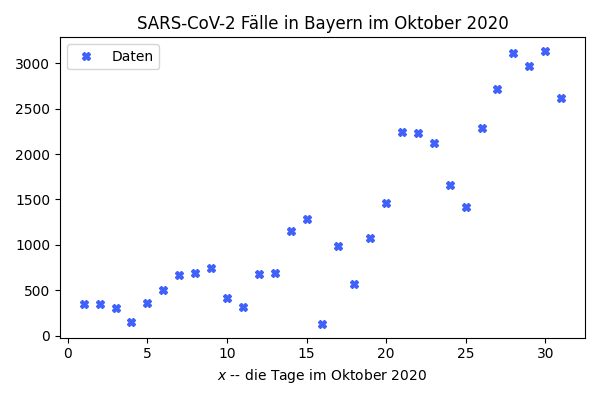
\includegraphics{bilder/02-cases.png}
\caption{Fallzahlen von Sars-CoV-2 in Bayern im Oktober
2020}\label{fig:cases}
}
\end{figure}

Wieder stellen wir uns die Frage ob wir \textbf{in den Daten einen funktionalen
Zusammenhang} feststellen können. Also ob wir die Datenpaare

\begin{quote}
(Tag \(x\), Infektionen am Tag \(x\))
\end{quote}

die wir als

\begin{quote}
(\(x_i\), \(y_i\))
\end{quote}

über eine Funktion \(f\) und die Paare

\begin{quote}
(\(x\), \(f(x)\))
\end{quote}

beschreiben (im Sinne von gut darstellen oder approximieren) können.

\hypertarget{rauschen-und-fitting}{%
\section{Rauschen und Fitting}\label{rauschen-und-fitting}}

Beim obigen Beispiel (und ganz generell bei Daten) ist davon auszugehen, dass die Daten \textbf{verrauscht} sind, also einem Trend folgen oder in einem funktionalen Zusammenhang stehen aber zufällige Abweichungen oder Fehler enthalten.

Unter diesem Gesichtspunkt ist eine Funktion, die

\begin{quote}
\(f(x_i)=y_i\)
\end{quote}

nicht zielführend. (Wir wollen Trends und größere Zusammenhänge erkennen und nicht kleine Fehler nachzeichnen.) Das zu strenge Anpassen an möglicherweise verrauschte Daten wird \textbf{overfitting} genannt.

Vielmehr werden wir nach einer Funktion \(f\) suchen, die die Daten näherungsweise nachstellt:

\begin{quote}
\(f(x_i)\approx y_i\)
\end{quote}

Hierbei passen jetzt auch Funktionen, die vielleicht einfach zu handhaben sind aber die Daten kaum noch repräsentieren. Jan spricht von \textbf{underfitting}.

Eine gute Approximation besteht im Kompromiss von \emph{nah an den Daten} aber mit wenig \emph{overfitting}.

\hypertarget{ansuxe4tze-fuxfcr-lineare-regression}{%
\section{Ansätze für lineare Regression}\label{ansuxe4tze-fuxfcr-lineare-regression}}

Um eine solche Funktion \(f\) zu finden, trifft Jan als erstes ein paar
Modellannahmen. Modellannahmen legen fest, wie das \(f\) im Allgemeinen
aussehen soll und versuchen dabei

\begin{enumerate}
\def\labelenumi{\arabic{enumi}.}
\item
  die Bestimmung von \(f\) zu ermöglichen
\item
  zu garantieren, dass \(f\) auch die gewollten Aussagen liefert
\item
  und sicherzustellen, dass \(f\) zum Problem passt.
\end{enumerate}

Jan bemerke, dass die ersten beiden Annahmen im Spannungsverhältnis zur
dritten stehen.

\textbf{Lineare Regression} besteht darin, dass die Funktion als Linearkombination

\begin{equation*}
f(x) = \sum_{i=1}^N w_i b_i(x)
\end{equation*}

von Basisfunktionen geschrieben wird und dann die \emph{Koeffizienten} \(w_i\) so bestimmt werden, dass \(f\) die Daten bestmöglich annähert.

\begin{quote}
Jan bemerke, dass \emph{bestmöglich} wieder \emph{overfitting} bedeuten kann aber auch, bei schlechter Wahl der Basis, wenig aussagekräftig sein kann. Der gute Kompromiss liegt also jetzt in der Wahl der passenden Basisfunktionen und deren Anzahl. (Mehr Basisfunktionen bedeutet möglicherweise bessere Approximation aber auch die Gefahr von \emph{overfitting}.)
\end{quote}

Typische Wahlen für die Basis \(\{b_1, b_2, \dotsc, b_N\}\) sind

\begin{itemize}
\tightlist
\item
  Polynome: \(\{1, x, x^2, \dotsc, x^{N-1}\}\) -- für \(N=2\) ist der Ansatz \emph{eine Gerade}
\item
  Trigonometrische Funktionen: \(\{1, \cos(x), \sin(x), \cos(2x), \sin(2x), \dotsc\}\)
\item
  Splines -- Polynome, die abschnittsweise definiert werden
\item
  Wavelets -- Verallgemeinerungen von trigonometrischen Funktionen
\end{itemize}

\hypertarget{fehlerfunktional-und-berechnung-der-approximierenden}{%
\section{Fehlerfunktional und Berechnung der Approximierenden}\label{fehlerfunktional-und-berechnung-der-approximierenden}}

Wir setzen nun also an
\begin{equation*}
f_w(x) = \sum_{i=1}^Nw_i b_i (x)
\end{equation*}
und wollen damit \(y_i \approx f_w(x_i)\) \emph{bestmöglich} erreichen (indem wir die Koeffizienten \((w_1, \dotsc, w_N)\) \emph{optimal} wählen. Bestmöglich und optimal spezifizieren wir über den Mittelwert der Abweichungen in der Approximation über alle Datenpunkte
\begin{equation*}
\frac{1}{N}
\end{equation*}

In unserem Falle, wollen wir annehmen, dass \(f\) eine lineare Funktion
(vielleicht auch noch als \emph{Gerade} bekannt)
\[f(x) = \theta_1 + \theta_2 x\] ist. Damit können wir sagen, dass

\begin{enumerate}
\def\labelenumi{\arabic{enumi}.}
\item
  \(f\) einigermassen einfach zu bestimmen ist (wir brauchen nur zwei
  Parameter \(\theta_1\) und \(\theta_2\))
\item
  wenn wir an Trends interessiert sind, sind lineare Funktionen eine
  gute Wahl
\item
  allerdings sind Prozesse meistens nichtlinear.
\end{enumerate}

Vor allem haben wir sicher oft gehört, dass die Virusausbreitung gerne
exponentiell verläuft, also zum Beispiel durch eine Funktion
\[g(x) = k_1 2^{k_2x}\] beschrieben werden sollte. Hier ist \(k_1\) ein
Skalierungsfaktor und \(k_2\) ein Parameter, der die Wachstumsrate
bestimmt.

In der Tat scheint die Annäherung der Datenpunkte aus Abbildung durch
eine Gerade nicht zielführend.

\begin{quote}
Allerdings sind exponentielle Zusammenhänge auf einer logarithmischen
Skala linear.
\end{quote}

Deshalb schauen wir uns die Daten über den Logarithmus (zur Basis \(2\))
der Infektionszahlen an

\begin{quote}
(Tag \(x\), \(\log_2\)(Infektionen am Tag \(x\)))
\end{quote}

Im Bild der Daten () kann Jan erkennen, dass eine Gerade vielleicht
(abgesehen von einigen Werten) ganz gut reinpassen könnte.

\hypertarget{lineare-regression-1}{%
\section{Lineare Regression}\label{lineare-regression-1}}

Die Methode der \emph{linearen Regression} besteht aus dem Anpassen einer
linearen Funktion (einer \emph{Geraden} im 2-dimensionalen Raum) an eine
Datenwolke. Aus den unendlich vielen Möglichkeiten die Funktion zu
definieren, wird die gewählt, die im Mittel den kleinsten Fehler
zwischen den Datenpunkten und der Funktionsbeschreibung erzeugt.

Für unser Beispiel der CoVID-19 Zahlen, können wir \emph{ad hoc} die
Parameter \(\theta_1\) und \(\theta_2\) bestimmen. Wenn es soweit ist,
werden wir die zugrundeliegenden mathematischen Konzepte und allgemein
gültige Formeln zur Lösung kennenlernen.

Konkret gehen wir davon aus, dass wir \(N\) Datenpunkte
\[(x_j,h_j), \quad j=1,2,3,\dotsc,N\] haben wobei \(x_j\) die Variable ist
und \(h_j\) das Merkmal dazu. In unserem Beispiel ist \(N=31\) (so viele
Tage hat der Oktober 2020), \(x_{10}=10\) wäre der 10. Oktober und
\(h_{10}\) der Logarithmus der Anzahl der am 10. Oktober registrierten
Fälle.

Und durch diese Datenpunkte wollen wir nun bestmöglich eine Gerade der
Form \[h(x)=\theta_1 + \theta_2 x\] legen. Bestmöglich bedeutet, dass
der Fehler über alle Datenpunkte gemittelt möglichst klein sein soll.
Dafür definieren wir zunächst den Fehler im Datenpunkt \(x_j\) als
\[e_j:= \frac 12 (h(x_j)-h_j)^2 = \frac 12 (\theta_1+\theta_2x_j -f_j)^2\]
wobei das Quadrat (u.a.) sicherstellt, dass alle Fehler positiv sind und
das ``\(\frac 12\)'' einfach ranmultipliziert wird um nachher beim Ableiten
einen Faktor zu sparen.

Und der gesammelte Fehler ist dann gegeben durch die Fehlerfunktion \(e\)
als die Summer aller Fehler:
\[e=e_1+e_2+\dotsc+e_N = \sum_{j=1}^N e_j = \frac 12\sum_{j=1}^N  (\theta_1+\theta_2x_j -f_j)^2\]

Jan kann erkennen, dass die Funktion \(e\) für verschiedene
\((\theta_1, \theta_2)\) verschiedene Werte annimmt und dass ein minimaler
Wert von \(e\) einen minimalen Fehler in der Approximation der Daten durch
\(h(x)=\theta_1+\theta_2 x\) bedeutet.

Und wie finden wir die Minimalstelle von \(e\) beziehungsweise die
optimalen \((\theta_1,\theta_2)\)? Fast wie in der Schule:

\begin{enumerate}
\def\labelenumi{\arabic{enumi}.}
\item
  die Funktion \(e\) ableiten,
\item
  eine Nullstelle der Ableitung finden.
\end{enumerate}

Dafür müssen wir erstmal verstehen, dass die Funktion eine Funktion von
2 Variablen ist (und dass das ein grosses Thema der Vorlesung werden
wird).

Fürs erste sei gesagt, dass Jan die Variablen \((\theta_1, \theta_2)\)
separat betrachten kann und danach ableiten und null setzen. Also nach
der Summen-- und der Kettenregel: \[\begin{aligned}
\frac{d}{d\theta_1} e(\theta_1, \theta_2) &= \frac 12 \sum_{j=1}^N  \frac{d}{d\theta_1} (\theta_1+\theta_2x_j -f_j)^2 = \frac 12 \sum_{j=1}^N 2(\theta_1+\theta_2x_j -f_j) \\
&= \sum_{j=1}^N (\theta_1+\theta_2x_j -f_j)\end{aligned}\] und
\[\begin{aligned}
\frac{d}{d\theta_2} e(\theta_1, \theta_2) &= \frac 12 \sum_{j=1}^N  \frac{d}{d\theta_2} (\theta_1+\theta_2x_j -f_j)^2 = \frac 12 \sum_{j=1}^N 2(\theta_1+\theta_2x_j -f_j)x_j \\
&= \sum_{j=1}^N (\theta_1+\theta_2x_j -f_j)x_j\end{aligned}\] abgeleitet
sodass das Nullsetzen \[\begin{aligned}
0&= \sum_{j=1}^N (\theta_1+\theta_2x_j -f_j) \\
0&= \sum_{j=1}^N (\theta_1+\theta_2x_j -f_j)x_j\end{aligned}\] uns zwei
Gleichungen ergibt, die (in aller Regel) die zwei unbekannten Parameter
\(\theta_1\) und \(\theta_2\) (eindeutig) bestimmen.

Mit den konkreten Zahlen von oben gerechnet (und auf 2 Nachkommastellen
gekürzt) identifizieren wir \[\theta_1^*=7.88, \quad \theta_2^*=0.12\]
als die optimale Wahl und damit \[h^*(x) = 7.88 + 0.12x\] als die beste
Gerade; Jan vergleiche Abbildung
\protect\hyperlink{fig:logtwo-cases-fitted}{3}.

Natürlich können wir mit \[y = 2^{\log_2(y)}\] auch das \emph{logarithmieren}
wieder rückgängig und auch die Ausgleichsgerade auf die lineare (nicht
\emph{logarithmische}) Datenskalierung transformieren
\[g(x) = 2^{\theta_1 + \theta_2 x} = 2^{\theta_1}\cdot 2^{\theta_2 x}\]
was uns mit den Parametern von oben die optimale Ausgleichskurve als
\[g^*(x) = 2^{7.88 + 0.12x} = 2^{7.88}\cdot 2^{0.12 x}=236.16\cdot 2^{0.12 x}\]
ergibt (dargestellt in Abbildung
\protect\hyperlink{fig:cases-fitted}{4}).

\begin{figure}
\hypertarget{fig:cases-fitted}{%
\centering
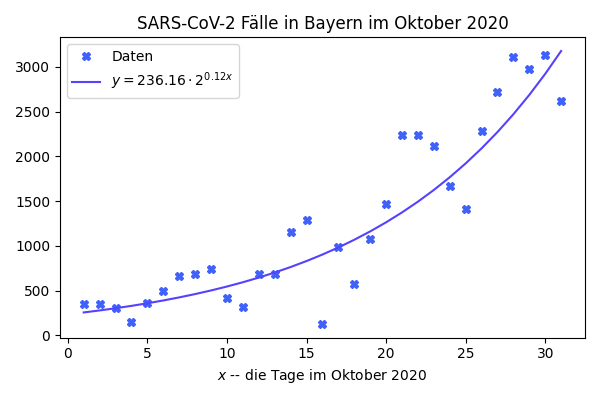
\includegraphics{bilder/02-cases-fitted.png}
\caption{SARS-CoV-2 Fälle in Bayern im Oktober 2020 und die mittels linearer
Regression auf der logarithmischen Skala bestimmte
Ausgleichskurve}\label{fig:cases-fitted}
}
\end{figure}

\hypertarget{sec:owo:mathematische-konzepte}{%
\section{Mathematische Konzepte in der Linearen Regression}\label{sec:owo:mathematische-konzepte}}

In diesem Beispiel haben wir schon einige Konzepte und Methoden benutzt,
die wir im Laufe der Vorlesung in allen Details kennenlernen werden.

Neben der grundlegenden Technik der \emph{linearen Regression} zur
Datenanalyse werden wir uns eingehend mit

\begin{itemize}
\item
  Elementarfunktionen (wie hier der Logarithmus und die
  Exponentialfunktion, aber auch trigonometrische Funktionen und
  weitere),
\item
  Differentiation und Integration von Funktionen und
\item
  dem Lösen linearer Gleichungssysteme
\end{itemize}

beschäftigen.

\end{document}
